\section{Part 4: counterexample acquisition premise}
\label{sec:part4}
Part 4 asks whether diverse physical hazards confidently missed by a small
predictor can improve held-out prediction per acquisition cost. The planned
comparison is stratified random sampling (R), uncertainty-guided mutation (U),
concentrated missed-hazard evolution (E), and diversity-preserving evolution (D).
Eight shared seeds, twelve new slots per method, eight confirmations and sixteen
common audit episodes give an 80-episode ceiling, conditional on predictor,
scene/reset and throughput feasibility. Policy and execution remain fixed; the
predictor observes execution without changing actions.

The ingredients have precedents: quality-diversity scenario
generation~\cite{fontaine2021scenarios}, uncertainty-based VLA annotation
acquisition~\cite{failurespot}, and counterexample-guided joint agent/critic
repair~\cite{boetius2024repair}. Their tasks and labels differ. No novelty or
optimizer-superiority claim follows from implementing these ingredients.

\subsection{Frozen causal target and direct predictor}
The offline protocol is pushed at \texttt{e66c2f9} before the Part 4 label audit;
the initial implementation follows at \texttt{9c9ccd9}. We restore and hash-check
the exact 24 Part 2/3 feature records and corresponding traces from private dataset
revision \texttt{f070abcb707b}. Its 3.34 GB raw archive passes SHA-256 verification.
Pinned native object scopes and tilt thresholds agree with numerical margins in
37,362 proposition-observation checks. Robot measurements, proposals, actual
environment inputs and query flags match their exact recorded trace entries.

The target is the first native uprightness violation of any protected object.
At observation $t$, predict its occurrence in the next $H=8$ actions while no
violation has yet occurred. A useful warning must occur in
$[\tau-8,\tau-4]$, where $\tau$ is first onset. At 20 Hz these specify a
0.4 s horizon and a 0.2 s deadline within the fixed-eight execution cadence.
History ends at $t$; actual executed commands stop at $t-1$. We exclude
already violated states, insufficient history and windows without eight real
future observations. There is no terminal padding or unsuccessful-episode label
substitution. One episode supplies at most one first-event warning denominator.

Fit-only PCA reduces the frozen two-camera DINOv2 features from 3,072 to 32 values.
The 255-dimensional primary input combines the current and four preceding
visual/robot observations, current proposed command, four previous actual commands,
known controller settings and query age. Controller metadata conditions the
historical A/B/C/D mixture. Privileged object states, monitor predicates, event time,
task identity, scene genes and future observations/actions are excluded.

Five episode-bootstrap MLPs each have one 64-unit tanh layer and exactly 500 Adam
updates of batch size 256. Bootstrap sampling is stratified by whole task.
Per-trajectory window contributions are capped at 256, with retained positives,
inverse-inclusion-weighted sampled negatives and equal episode mass before class
balancing. Fixed L2 logistic models provide full-input and visual-only references.
Platt probability calibration and each operating threshold use the common
calibration task. Architecture, seeds, updates, targets and thresholds are not
retuned using development outcomes. Encoder, dynamics and VLA weights stay fixed.

\begin{table}[t]
\caption{Part 4 exposed historical development data. Positive windows are
correlated within the first event; the Part 3 audit is not a fresh Part 4 audit.}
\label{tab:part4-support}
\begin{tabular}{lrrrr}
\toprule
Group & Tasks & Episodes & Events & Pos./windows \\
\midrule
Fit & 2 & 16 & 4 & 32/8,390 \\
Calibration & 1 & 4 & 3 & 24/2,584 \\
Development & 1 & 4 & 1 & 8/2,237 \\
\bottomrule
\end{tabular}
\end{table}

Fitting uses tasks 0039/0010, calibration 0046 and development 0006. All four
fitting events occur on task 0039, failing the minimum two event-task criterion.
Development has one event, failing its minimum two episode criterion
(Table~\ref{tab:part4-support}). Missing support remains inconclusive. All task
variants stay in one group, the fresh final audit is not selected or opened,
and released VLA pretraining overlap remains unknown.

\subsection{The operating point fails to generalize}
The primary alarm threshold is .02995514. Its calibration false-alarm rate is
4.9801\% when episodes receive equal weight; pooled counts are 110/2,560,
or 4.2969\%. Low risk means probability at most .1. Low disagreement means
uncalibrated member-probability standard deviation at most .00204003, the
calibration negative-window 25th percentile. Calibration of the mean and the
disagreement statistic are recorded separately.

\begin{table}[t]
\caption{Part 4 development prediction at operating points frozen on calibration.
False alarms are pooled negative windows. Every model warns on the one event;
this alone does not establish a useful trade-off.}
\label{tab:part4-warning}
\begin{tabular}{lrrr}
\toprule
Predictor & AUROC & AP & False alarms \\
\midrule
MLP ensemble & .8345 & .0121 & 2,045/2,229 \\
Full logistic & .8845 & .0165 & 948/2,229 \\
Visual logistic & .9735 & .4258 & 1,575/2,229 \\
\bottomrule
\end{tabular}
\end{table}

Primary average precision (AP) exceeds the .003576 positive-window prevalence but
fails the frozen .05 minimum. Its 91.75\% negative-window false-alarm rate exceeds
the .15 maximum (Table~\ref{tab:part4-warning}). Every development episode has a
false alarm, 4/4, as does every calibration episode, 4/4. Always-alarm also misses
zero events but alarms on all 2,229 negative windows; always-safe misses 1/1 events
without false alarms. The observed 0/1 missed timely warnings therefore cannot
validate this operating point. The visual-only reference ranks better but still
alarms on 70.66\% of negative development windows; it is not substituted after the
gate fails (Figure~\ref{fig:part4-tradeoff}).

\begin{figure*}[t]
\centering
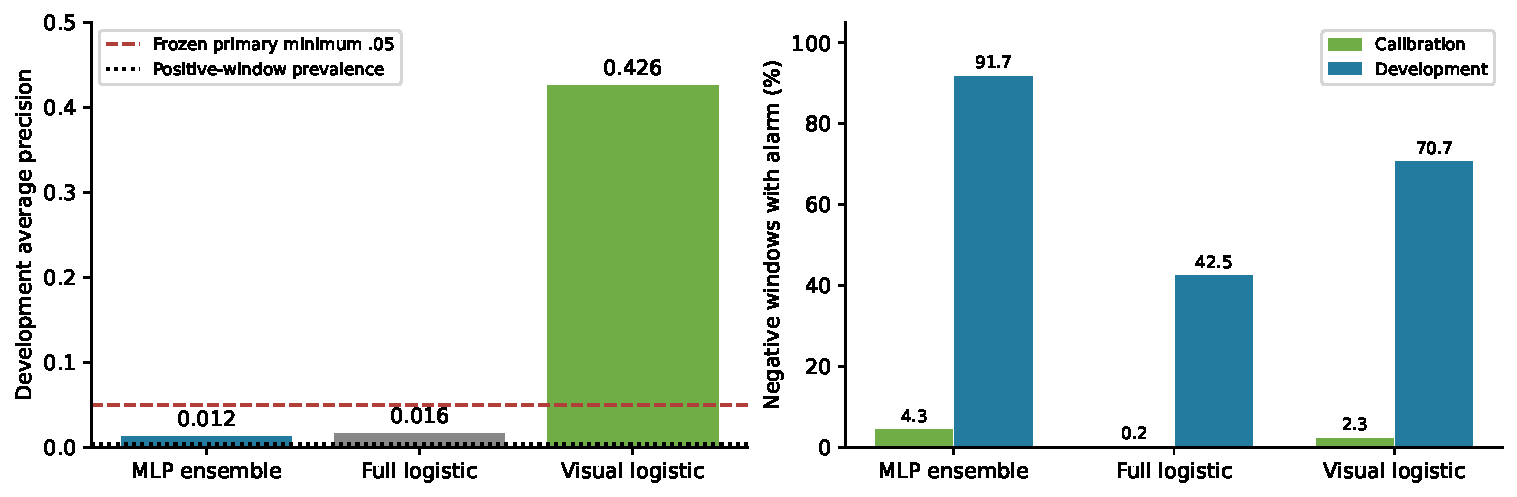
\includegraphics[width=.97\textwidth]{warning-tradeoff.pdf}
\caption{Part 4 discrimination and actual false alarms on exposed development
data. The visual-only ablation ranks the one event better, while its frozen
operating point still has excessive false alarms. Eight positive windows come
from one event, not independent failures. Calibration columns show pooled rates;
threshold selection weights episodes equally.}
\Description{Primary and full-logistic average precision are .012 and .016,
versus .426 for visual logistic. Development false alarms are 91.7, 42.5 and
70.7 percent. These rates are much higher than their calibration values.}
\label{fig:part4-tradeoff}
\end{figure*}

The primary misses 3/3 calibration events. One is a qualifying low-risk miss:
\texttt{part3-record-b0-C}, bowl\_69 onset 843, with deadline probability .0119821
and disagreement .00165808, giving descriptive quality .988018. The other two
misses have greater disagreement. The sole development event, teacup\_73 onset
307 in \texttt{part3-record-b3-B}, warns eight actions early, with deadline
probability .113333 and disagreement .196481. It is not a confident miss; all
295 negative windows in that episode alarm. The calibration case neither proves
reproducible acquisition nor supplies independent development support
(Figure~\ref{fig:part4-timelines}).

\begin{figure*}[t]
\centering
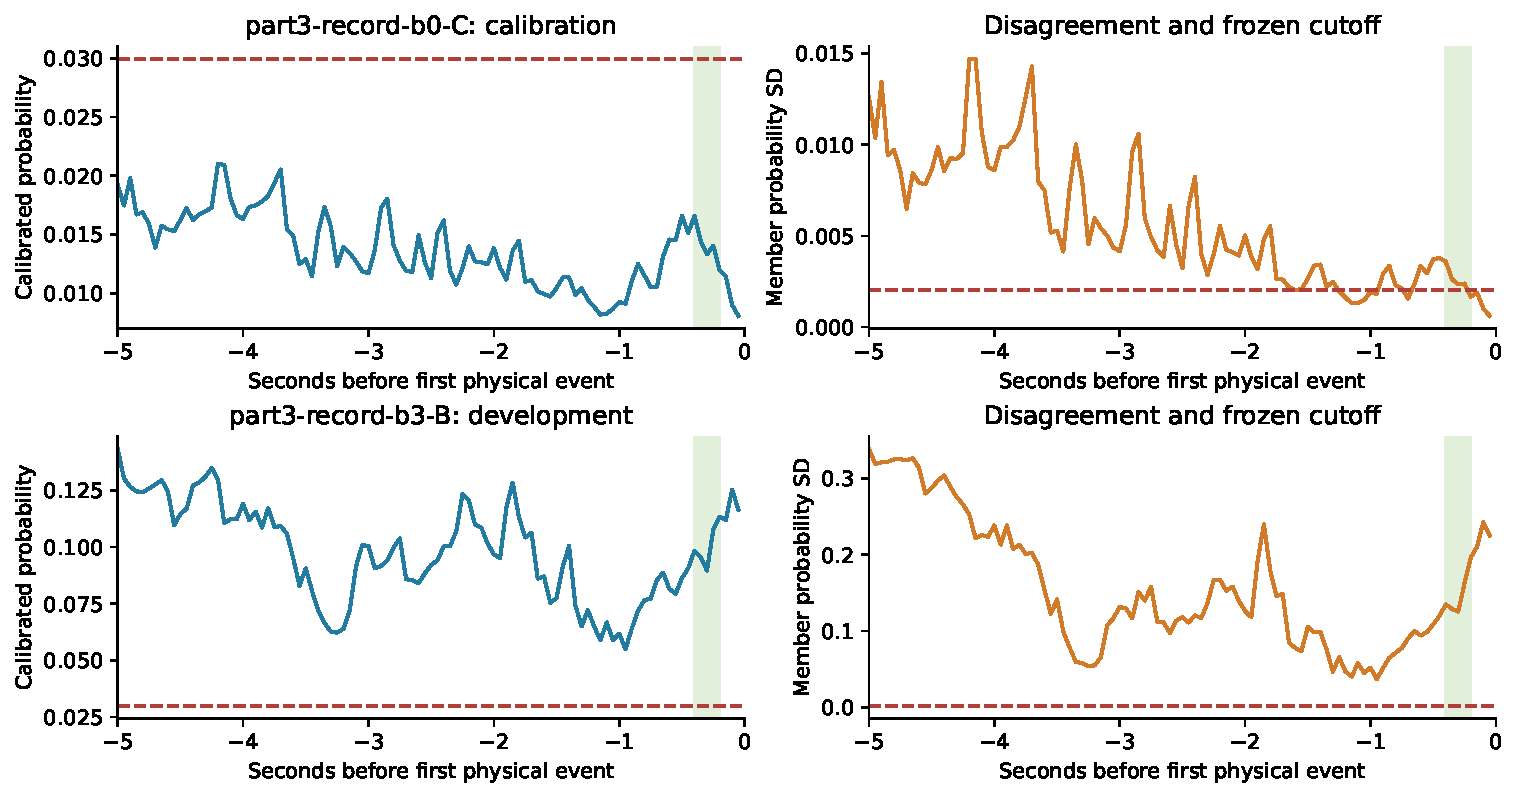
\includegraphics[width=.93\textwidth]{warning-timelines.pdf}
\caption{Historical calibration low-risk miss (top) and development event with
excessive alarms (bottom). Green marks the eligible 0.4 to 0.2 s warning interval;
red dashed lines show frozen probability and disagreement cutoffs. Scores end
before the first event. No hypothetical action branch or new physics is used.}
\Description{The calibration miss remains below the alarm threshold. Development
probabilities exceed the threshold throughout this displayed five-second prefix,
and disagreement is much larger than the low-disagreement cutoff.}
\label{fig:part4-timelines}
\end{figure*}

The frozen gate is \texttt{failed\_discrimination}, with additional support and
confident-miss failures. Shared-initial rescue requires discrimination to pass,
so those eight episodes are ineligible. Physical scene/reset engineering, all
48 acquisitions, eight confirmations, repair and sixteen audit episodes remain
unstarted. Empty stage receipts retain those distinctions; there is no generated
scene, archive elite, repaired predictor, recurrence rate or held-out repair result.
The CPU acquisition kernels and matched-update helper are implemented, with tests
for bookkeeping and information isolation, but have no physical validation here.

\subsection{Costs and preservation}
Part 4 adds zero simulator attempts, controls, physics steps, VLA queries or encoder
calls. The 24 reused donors retain their original 18,657 controls, 3,165 queries and
114,006 known post-subscription physics ticks, charged once. Their physical outcomes
are 14 safe completions, one unsafe completion, two safe unfinished and seven
violating unfinished episodes. Pre-subscription physics remains unknown; the
uprightness prediction target does not replace the other native physical outcomes.
Uprightness violations occur in 4/16 fitting, 3/4 calibration and 1/4 development
episodes. Spill occurs in 3/4 calibration episodes; no donor has a native drop
violation. Types can overlap. Task-specific proposition names are resolved from
their pinned definitions and the resulting violation flag matches every audit.

New fitting uses 2,500 MLP updates and 640,000 sampled windows. Scoring evaluates
66,055 ensemble-member windows and 26,422 reference windows. One worker fails after
training when reloading a partially reconstructed PCA estimator. Prediction resumes
from identical hash-verified weights using the explicit saved affine transform;
no second fit or model search occurs. The failed attempt and time are retained.

The existing replacement allocation is single-RTX-3090 instance 56676451, beginning
19 October 05:28:29.253 UTC, rather than the proposed 4090/5090. The physical cutoff
is 12:28:29.253 UTC and hard stop 13:28:29.253 UTC. All preparation, implementation,
reporting and idle time count from the original provider start, with an independent
supervisor-managed deadline guard. This preparation base is not a validated ManiGuard
stack, and no simulation-throughput or reset-repeatability claim is made.

Eight two-camera event strips and two 101-frame, 20 Hz videos use individually
hash-checked historical RGB. They show warning start, deadline, native onset and
post-onset observations without replaying physics. Own weights and evidence are
separately private, revision-pinned and download/hash verified; full identifiers
are in the Part 4 export and gallery linked from the paper README. Final
preservation and provider state are recorded separately from scientific termination.
This bounded result supplies no evolutionary acquisition or repair-efficacy claim.
